\startchapter{Mixture} \label{ch:5}
\section{Description}

In Chapter \ref{ch:4}, experiments indicate that for one kind of molecule at interfaces, even combine all the three kinds of spectral information, the LP model constructed can not return the target composition for most cases. The existing spectral information is not adequate to obtain an unique solution for the composition of molecule coordination distribution at interfaces. Multiple compositions can build spectra that are exactly the same as the target ones. These compositions are return by different LP models that using different amount of spectra information. For each LP model, because of the numerical limitation, each LP model returns an optimal solution in the composition. \\


%In Chapter \ref{ch: 4}, we have learned that even the LP models have combined the data information from three spectra techniques, it is impossible to get the exact coordination distribution for one kind of molecule at interfaces.



All the spectral information from three techniques has been extracted in building the LP model for one single kind of molecule at interface. The spectral information is limited in the goal of obtaining the target composition for one molecule. However, that's one factor of our focus. Next step, the focus is moved to the study of multiple different molecules at interfaces. For this mixture of different molecules, will LP models built with different spectral information help to return the given target composition. If any of the LP models success in obtaining the target composition, its accuracy is the key factor for the study as well. \\

%This has restricted our LP model's further development, as seemly there is no more information from the spectroscopy techniques we could extract further to refine our LP models.(Any information I need to back up this statement???) It also constraints us to further study the limitation of our LP models. Therefore, we would like to take a step back, considering a mixture of different molecules. We want to know if the LP models we built with different spectroscopy information can help us to knowing the composition of a pool of mixed molecules. Same as Chapter \ref{chapter:4}, given a target spectra, would any of our LP models tell us the accurate composition of the mixture. With the ones that are capable of achieving this, we want to further know each LP model's accuracy in turn of times that it gets the correct composition.

\section{Experiments}

In order to achieve the above goals, further experiments are needed. These experiments have the following common settings. \\

First of all, there are six different amino-acids in the mixture: methionine, leucine, isoleucine(ile), alanine, threonine and valine. For each amino acid, only $\theta$ difference is considered, the other two Euler angles are integrated. Each amino acid molecule has 9 candidates in the mix, which are $\theta$ of the following degrees: $0^{\circ}$,  $10^{\circ}$, $20^{\circ}$, $30^{\circ}$, $40^{\circ}$, $50^{\circ}$, $60^{\circ}$, $70^{\circ}$ and $80^{\circ}$. Because the SFG spectra for $\theta$ equals $90^{\circ}$ is a straight line, this candidate is excluded in the experiments. As a result, there are 54 candidates in the mix. \\

Secondly, target composition needed to be generated. Two steps are operated: randomly pick one candidate from each amino acid's 9 candidates, then randomly generate a percentage for the selected candidate. The target composition is made up of $6$ randomly selected candidates, with each one coming from six different amino acids. The rest $48$ candidates contain $0$ percentage in the target composition. The total percentage of 6 selected candidate makes 100\% component of the mix. \\

Third, we need to generate the IR, Raman and SFG spectra for all the $54$ candidates' and the target. \\

%The LP model built for each experiment will still have all the 54 candidates' spectra in the model to study if the LP model will give a composition matched to what we have generated. 

%In order to study which spectroscopy technique is more efficient in obtaining coordination information, we need to set up different experiments. In these experiments, the basic setting is the same as described above. The difference is that each LP model for an experiment is constructed using different spectra's information. To set up for the comparison, we have the following group of experiments:

For each experiment in the experiment set, it contains different spectroscopy information as shown in Table \ref{tab:5.1}. For E1 in the table, candidates' IR x and z projections spectra are obtained, as well as target's IR x and z projections spectra generated by dot product of the target composition and all the candidates' spectral data. Then the corresponding LP model is conducted. Therefore, the LP model for E1 only contains IR information.\\

%Table 5.1 displays the detailed setting for the experiment group. 

\begin{table}\tiny \label{tab:5.1} 
\begin{center}
\begin{tabular}{| l | l | l  }
\hline
Experiment Index & Spectrum Information \\
\hline
E1 & x and z polarized IR spectra\\
\hline
E2 & xx, xy, xz and zz polarized Raman spectra \\
\hline
E3 & yyz, yzy and zzz polarized SFG spectra \\
\hline
E4 & x and z polarized IR spectra; xx, xy, xz and zz polarized Raman spectra \\
\hline
E5 & x and z polarized IR spectra; yyz, yzy and zzz polarized SFG spectra   \\
\hline
E6 & xx, xy, xz and zz polarized Raman spectra; yyz, yzy and zzz polarized SFG spectra \\
\hline
E7 & x and z polarized IR spectra; xx, xy, xz and zz polarized Raman spectra; yyz, yzy and zzz polarized SFG spectra \\
\hline
\end{tabular} 
\end{center}
\caption{Detailed Experiment Group Setting} 
\end{table}	

%or all the experiments in this group, the composition for the target spectrum is the same.  For each amino acid, we randomly select one  from the 8 candidates, the assigned a random percentage. This composition is generated before all the experiments are run.


%Then we use the spectra data to generate the according LP model. Therefore, we say this LP model only contains IR information.
Same idea for E2, it contains Raman's xx, xy, xz and zz four projections spectral information. E3 only contains SFG's yyz, yzy and zzz three projections spectral information. \\

Start from E4, spectral information from different spectroscopy techniques are combined. For E4, IR's x and z projections are combined with Raman's xx, xy, xz and zz four projections spectral information in the LP model. For E5, IR's x and z projections are combined with SFG's yyz, yzy and zzz three projections spectra information. For E6, Raman and SFG spectral information are incorporated. At the end, for E7, all three spectral information are put together: IR, Raman and SFG. \\

The LP models for each experiments are using the same formula as shown in Equation \ref{eq:3.4}. Because every experiment is built with different spectral information, each LP model is different. \\

Finally, this experiment set is run 100 times in order to see which experiment in Table \ref{tab:5.1} gives us the target composition with the highest accuracy. This accuracy is measured by the time of each experiment hits the target composition. The scoring mechanism to measure a return composition matches to the target one is described in the section of Scoring Methods. \\

\section{Scoring methods}

At first glance, the sum of residuals between the spectra composed by the return composition and the target one, is considered to measure the accuracy of the return composition. However, for most experiments conducted earlier, the spectra generated by the return composition are almost identical to the one created by the target one.   This sum of residuals is also negligible. It is impossible to use it as a scoring criteria. \\

The only way to measure the accuracy of the return composition, is to compare it with the target one. Therefore, calculating the sum of the residual between the target composition and the return one directly is the fastest way to evaluate the accuracy of each experiment. The shortage of this approach is that it cannot be used to measure in real life where the target composition is unknown. However, for current experiments, this approach can be a way to evaluate the different spectroscopy techniques. In addition, a glance of which spectroscopy technique have the highest sensitivity can be studied. \\

%we need a way to eventually evaluate each approach. We were thinking by using the sum of residuals between the spectra that composed by return composition and the one composed by target composition. However, these two spectra are almost identical, therefore, the sum of residuals is almost negligible. It is impossible for us to use it as a scoring criteria.

%We came up with an idea, what if we consider the difference between return and target composition itself, so that it can help us to distinguish which technique is more sensitive. And we know that this method has its shortage that it can not be applied to real life where that we do not know the target composition of the mix. However, for current situation, it is just a way for us to evaluate the different spectroscopy techniques.

The return composition of each experiment in the experiment set will be obtained for each run. Each return composition is compared with the target one to calculate the sum of the residual. If the residual is smaller than a certain threshold, which is $1e-7$, the return composition is considered to be the same as the target one. \\

%For each run of the experiment group, we obtain the composition returned by each experiment. And based on the return composition, we calculate how many times each experiment returns the same composition as the target one. In result, we have Figure \ref{fig:5.1} as shown below.

\begin{figure}[!ht] \label{fig:5.1}
\centering
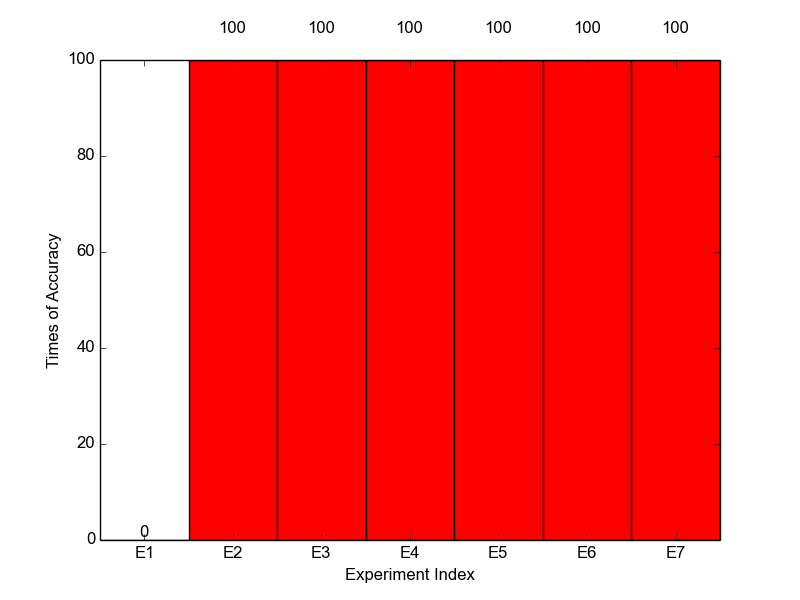
\includegraphics[scale=0.7]{Figures/accuracy_pecent_result8_mixture.png}
\caption{Accuracy analysis for experiments considering a mixture of amino acids with candidates from $0^{\circ}$ to $80^{\circ}$ on $\theta$ for each amino acid} 
\end{figure}

After running the experiment set for 100 times, the interesting result is shown in 
Picture \ref{fig:5.1}. E2, the return composition of the LP model constructed using Raman's four projections' spectral information meets the target composition 100 times. This means that within this set of experiments, Raman is sufficient enough to figure out the correct composition for the target spectra. Moreover, the accuracy is 100\%. \\

E3 is the LP model constructed using SFG's three projections' spectral information. Same as E2, its spectral information is as abundant as Raman's spectra for this set of experiments. The accuracy is 100\% as well. \\

E4, E5, E6, and E7, as they either contain information of Raman, or SFG, or both. Therefore, the corresponding LP model can help to get the desire target composition with same accuracy as E2 and E3. \\

The only exception is E1. The accuracy is not as high as the others. The accuray of LP model constructed using IR's two projections' spectral information is 0. The reason, for the LP model built using only IR spectral information having low performance, can be that the spectral information is not sufficient to obtain the target composition. 
%This makes us wonder how come the performance of the LP model that merely use IR spectra be so low? And even if the performance is low, can we still extract any valuable information that indicates IR could still be useful in some cases? \\

When this experiment set is re-run 100 times, only E1's returned composition is analyzed and focused. For each run, x and z projected IR spectra are constructed together both by the returned composition and the target one. The result is that: these two projections' spectra conducted by the two different compositions are almost identical to each other for every run. As an example, a random run is picked, then the two spectra are plotted in Figure \ref{eqn:5.1}. The spectrum plotted by the return composition is identical to the one plotted by the target composition. This indicates that the optimum composition returned by the LP model conducted with only IR spectral information has achieved its best in obtaining a composition that best fit the target spectra. 
%However, with limited information, the LP model cannot further distinguish the candidates, therefore, make it impossible to obtain an even more accurate composition. Moreover, because our candidates for each amino acid are quite similar to each other by just looking at the spectra. It is very possible that there are more than one possible compositions can perfectly re-construct the target spectra.  Therefore, we would need more constraints to refine our candidates' selection for the target composition. 

(TODO: rewrite or remove this paragraph) Comparatively, SFG has three unique projections, and Raman has four unique projections. From each projection's spectrum, we evenly select 200 data points. This means that one more projection will bring in 200 more constraints or 400 more (if we take the absolute sign off) constraints to the LP model. This would make a huge in LP model, in term of further refining the candidate selection in target composition. However, it is still too early for us to say that Raman has more coordination information because it has four unique projections. Because for Raman's any projection, the spectrum of candidate with $\theta$ equals to one degree is identical to the one of candidate with this $\theta$ degree's complementary. For example, the Raman spectra for candidate with $\theta$ of $10^{\circ}$, is the same as candidate with $\theta$ of $170^{\circ}$. And for IR, it is the same case. Only SFG tells the differences between these two degrees, as the spectra for candidate with $\theta$ of one degree is symmetric to its complementary along wavelength. \\

\begin{figure}[!ht] \label{fig:5.2}
\centering
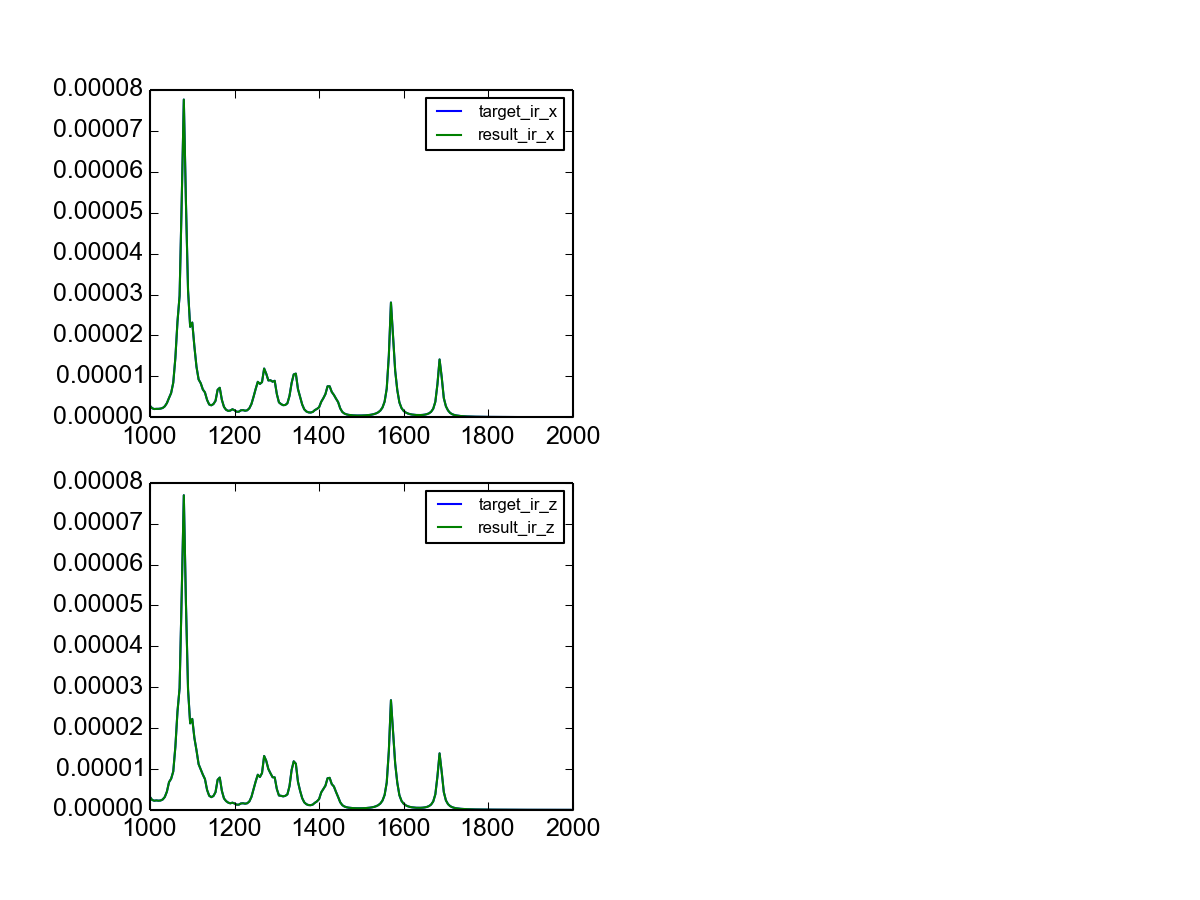
\includegraphics[scale=0.7]{Figures/result_target_plotting_ir16.png}
\caption{IR Spectra Plotted by Result Composition and Target Composition} 
\end{figure}

%This shows that with the information that IR spectra have, it is not sufficient to abstract the orientation distribution of the mixed molecules at surface in this case.

%However, Raman or SFG only is good enough to obtain the desire result.

To further study the capacity of the LP models for the mixture of molecules,the candidate pool is expanded from $0^{\circ}$ to $180^{\circ}$ on the value of $\theta$ degree. Therefore, each amino acid has 18 candidates. In total, there are 108 candidates in the mix. The same set of experiments in Table \ref{tab:5.1} is used. The only different is to to randomly select one candidate from 18 candidates, instead of 9. All 108 candidates' IR, Raman and SFG spectra are needed to be generated. After 100 runs, Figure \ref{fig:5.3} indicates the results. The accuracy for E1 is still low. This is not surprising as the complexity of the candidates has increased. Moreover, IR spectra for candidate with $\theta$ of one degree is identical to the one with $\theta$ of this degree's complementary, as shown in Figure \ref{fig:5.4}. This also increases the difficulty for the LP model constructed by using IR spectral information to return the correct composition. \\
%Then we run the same group of experiments in Table \ref{tab:5.1} 100 times. The only differences are in the general setting. For target composition for each experiment group, we need to randomly select one candidate from 18 candidates, instead of 9. What's more, we need to 108 candidates' IR, Raman and SFG spectra. The goal is to study which experiment in Table \ref{tab:5.1} will give us the highest accuracy with current candidate pool. In return, we have Figure \ref{fig:5.3} showing the experiment result. 

\begin{figure}[!ht]
\centering
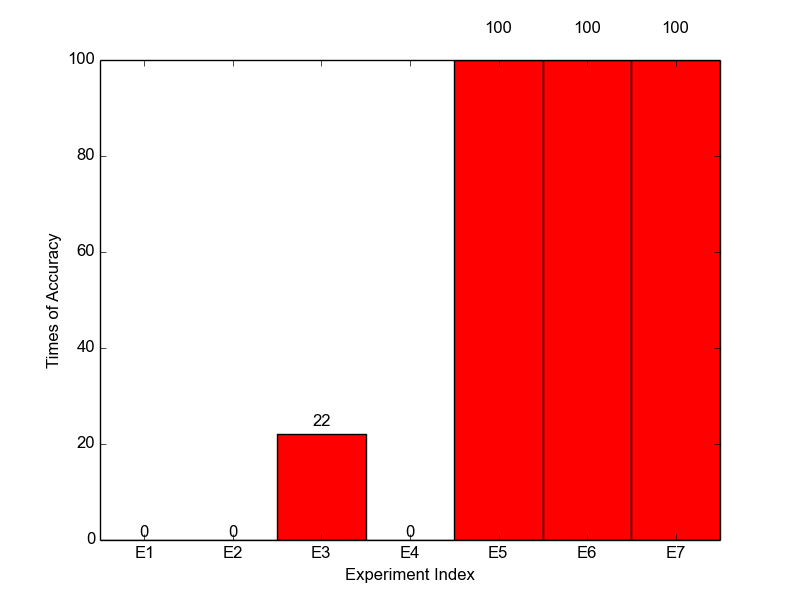
\includegraphics[scale=0.7]{Figures/accuracy_pecent_result10_mixture.png}
\caption{Accuracy analysis for experiments considering a mixture of amino acids with candidates from $0^{\circ}$ to $180^{\circ}$ on $\theta$ for each amino acid} \label{fig:5.3}
\end{figure}

However, it is very interesting to observe that the accuracy for E2 has dramatically dropped. This is because the Raman spectra for one candidate with $\theta$ on one degree is identical to the one with this degree's complementary. Further explanation  will be provided on this reason. \\

Also from Figure \ref{fig:5.3}, the accuracy for E3 is no longer high neither. After increasing the candidate number from 9 to 18 for each amino acid, the complexity of the corresponding LP model has increased. From each projection, 200 data points are selected from both target and candidates' spectra. Therefore, there are same number of constraints, in contrary, the number of candidates are twice bigger as before. Although the extra candidates' SFG spectra are symmetric along wavelength which may greatly increase the uniqueness of the candidates. However, the spectral information is still insufficient to converge the composition to the target one. \\
% in the LP model, the objective function here is to minimize the sum of each data point's absolute subtraction between the target spectra and the one generated by candidates' spectra and return composition. Because of the nature(!!!need to expand a bit), composition return by E3's LP model can be far off the target one in the solution dimension if we do not have enough constraints.\\

%The reason for E4 to have low accuracy could be the same as E2. Even combining IR and Raman, there is no way for us to distinguish the candidates that with $\theta$ and the one with this degree's complementary, for each amino acid. We will compare the return compositions of E2 and E4 to see if there is any improvement after combining IR to Raman.\\

The good result starts to emerge when we combine IR with SFG or Raman with SFG. Figure \ref{fig:5.3} shows that E5, E6, E7 all have 100\% accuracy. This phenomenon may not be hard to explain at the first glance. SFG helps to distinguish a candidate from its complementary on $\theta$ value. Extra spectral information coming from IR or Raman helps to further refine the LP model which can converge the return composition to the target one. \\
%This may not be hard to explain even in the first glance, when you combine IR with SFG, we have IR's 2 projection and SFG's 3 projection spectra. From SFG, we have information to distinguish from a candidate and its complementary $\theta$ degree. With the help of IR, we have enough information to construct the constraints in the LP model. Let along mentioning the combination of Raman and SFG, as Raman has 4 projection spectra where we can extra more data points to further refine the model. \\
Although the accuracy of E1 is low when each amino acid's candidates spread from $0^{\circ}$ to $180^{\circ}$ on $\theta$. There are still some interesting result buried in the return composition: for each amino acid, the percentage assigned to it is correct, however, the candidate presented may be the one with correct degree, or the one with correct degree's complementary. Among 100 runs, randomly select one run of the experiment set as an example. \\
  
%What I want to study further is the result of E2, the one with the LP model constructed by only Raman spectra information. And here is the interesting thing we have observed from the return composition of E2: the percentage value of possibly existing candidate for each amino acid is correct, but this possibly existing one may not be the correct one all the time, it could be correct one's complementary on $\theta$.
%for each amino acid's existing candidate in target composition, we can tell it is either the candidate with the exact $\theta$ degree or the candidate with this exact $\theta$ degree's complimentary. 
Figure \ref{fig:5.4}is the target composition and Figure \ref{fig:5.5} is the return composition for E2. Figure \ref{fig:5.6} is the return composition of E6. From all these three figures, when extracting the non-zero values to generate a list, these three lists are the same. However, when overlapping Figure \ref{fig:5.4} with Figure  \ref{fig:5.5}, the position of each non-zero value is not identical. For example, value of $0.299586$ appears at $\theta$ of $150^{\circ}$ for Valine in Figure \ref{fig:5.4}. In Figure \ref{fig:5.5}, it appears at $\theta$ of $30^{\circ}$ for Valine. Same for value of $0.021196$, $0.00662804$, $0.000642609$, and $0.00789$. The LP model of E2 fails to tell which candidate is the exact one between the correct one and its complementary on $\theta$'s degree sometimes. This observation is a general case across all the experiment groups. From E6, as long as the spectra data from SFG is plugged into the LP model, the return composition is the same as the target one. \\


\begin{figure}[!ht] \label{fig:5.4}
\centering
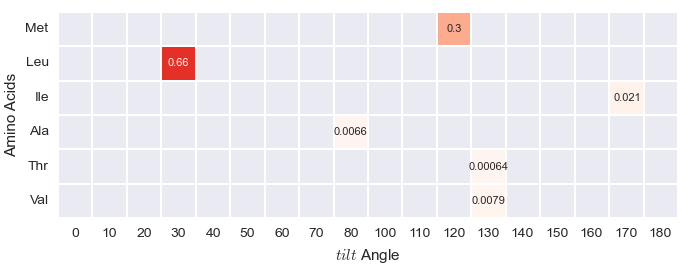
\includegraphics[scale=0.4]{Figures/mixture_target_composition_for_one_run_theta_0_180.png}
\caption{Target Composition for One Run of Mixed Amino Acids with $\theta$ Expanded from $0^{\circ}$ to $180^{\circ}$} 
\end{figure}

\begin{figure}[!ht] \label{fig:5.5}
\centering
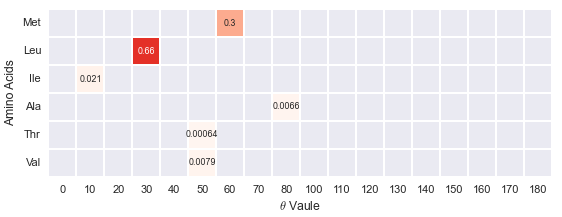
\includegraphics[scale=0.4]{Figures/mixture_return_composition_of_E1_for_one_run_theta_0_180.png}
\caption{Return Composition of E1 for One Run of Mixed Amino Acids with $\theta$ Expanded from $0^{\circ}$ to $180^{\circ}$ on $\theta$} 
\end{figure}

\begin{figure}[!ht] \label{fig:5.6}
\centering
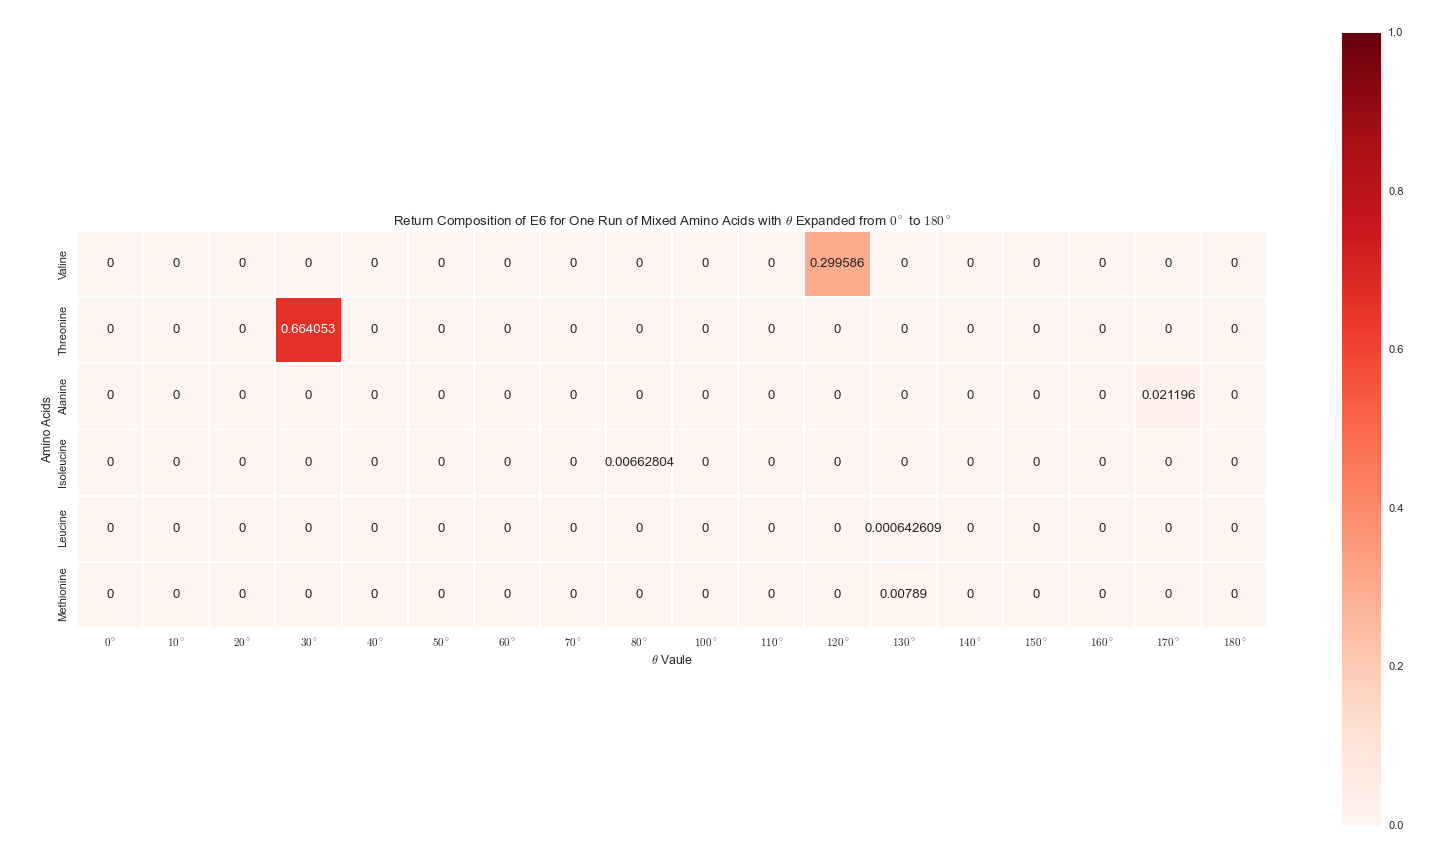
\includegraphics[scale=0.4]{Figures/mixture_return_composition_of_E6_for_one_run_theta_0_180.png}
\caption{Return Composition of E6 for One Run of Mixed Amino Acids with $\theta$ Expanded from $0^{\circ}$ to $180^{\circ}$ on $\theta$} 
\end{figure}

%We randomly take one group of experiment run as an example, Array \ref{eqn:5.1} is the target composition that we generated randomly. And Array \ref{eqn:5.2} is the return composition of E2, Array \ref{eqn:5.3} is the return composition of E6. When comparing Array \ref{eqn:5.1} with Array \ref{eqn:5.2}, if we take the percentage value of each existing candidate in the target composition and the composition returned by E2, the two arrays are identical. However, what's different is the existing candidate for each amino acid may not be correct. For example, in target composition, we have 0.299586 of candidate with $\theta$ of $120^{\circ}$ for methionine, but the one return by E2, has 0.299586 of candidate with $\theta$ of $60^{\circ}$ for methionine. $60^{\circ}$ and $120^{\circ}$ are complementary to each other, which means the Raman spectra for these two candidates of methionine are identical. E2's LP model may take each one of them as an existing candidate in the return composition, and this may not be surprising. In the result, it is the same case for isoleucine(ile), alanine, threonine and valine. The LP model of E2 fails to tell which candidate is the exact one between the correct one and its complementary on $\theta$'s degree. This observation is a general case across all the experiment groups. What's more, from E6, we know as long as we plug in the spectra data from SFG into our LP model, we can obtain the correct composition same as the target one. \\

From the above analysis, E2 appears the ability of limiting the number of candidates to 2 for each amino acid. These two candidates are complementary on $\theta$ degree, with one of them to be the correct one for the target composition. The return composition of E4 is the same as the one of E2, which means IR spectra information is not helping in this case. Spectral information from SFG is needed in order to study the cases that having $\theta$ expanded from $0^{\circ}$ to $180^{\circ}$.\\

%Experiment 2: the LP model that constructed by using only four projections of Raman spectra does not contain enough information any more for the current case. 

%Experiment 3: The information coming from SFG three projection is not completely sufficient, however, it is much better than IR or Raman. The underline reason is actually quite obvious, because the IR spectrum for $\theta = 0^{\circ}$ is the same as the one for $\theta = 180^{\circ}$, so as for Raman, the spectra of $\theta = 0^{\circ}$ and $\theta = 180^{\circ}$ are identical at every projection. Contrarily, the SFG spectra for them are symmetric. The following three pictures display Alanine's IR z projection, Raman zz projection and SFG zzz projection spectra. As shown, the IR and Raman spectra for theta with 0 degree and 180 degree are same, but for SFG, their are symmetric.

\begin{figure}[!ht] 
\centering
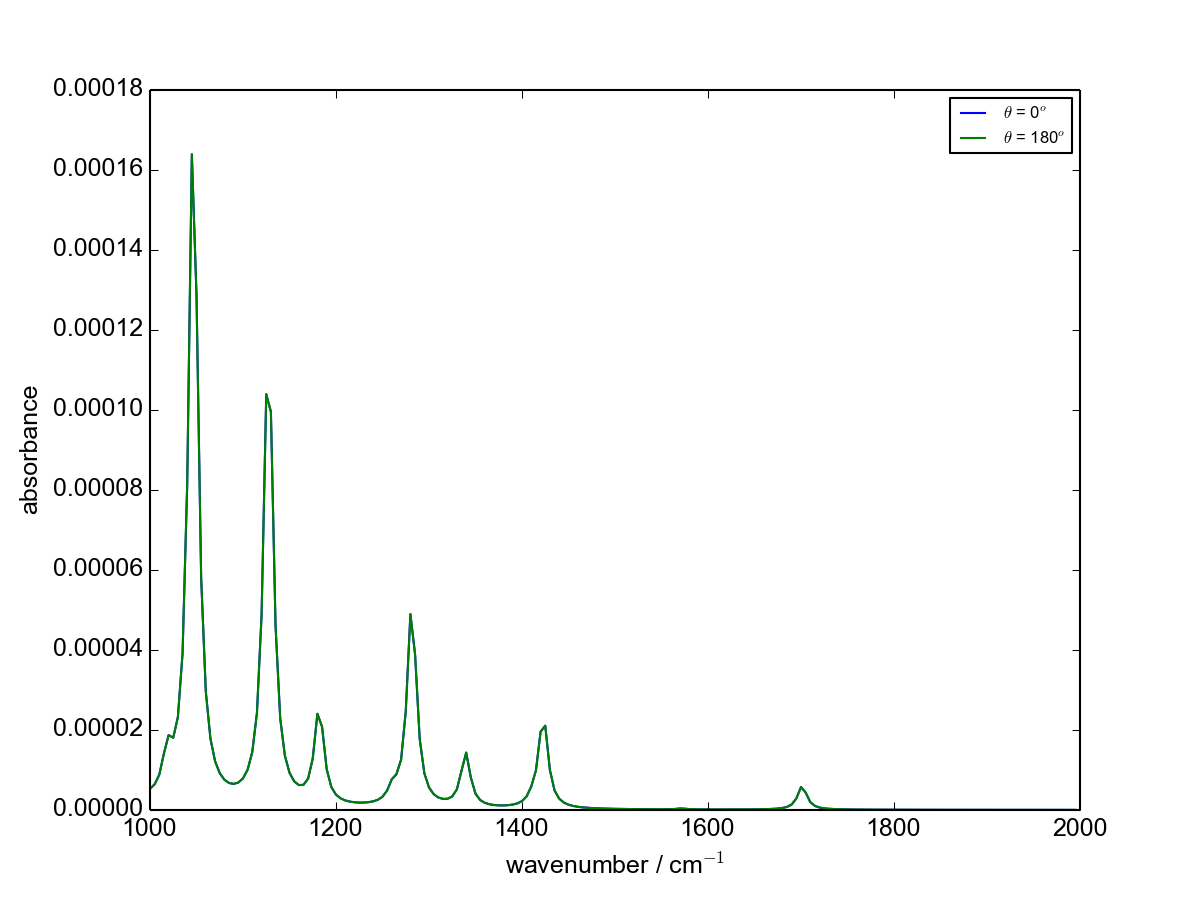
\includegraphics[scale=0.7]{Figures/Ala_candidates_plotting_ir_z_2.png}
\caption{IR z projection spectrum for Alanine Candidate with $\theta$ of $0^{\circ}$ is identical to Alanine Candidate with $\theta$ of $180^{\circ}$} \label{fig:5.7}
\end{figure}

\begin{figure}[!ht] 
\centering
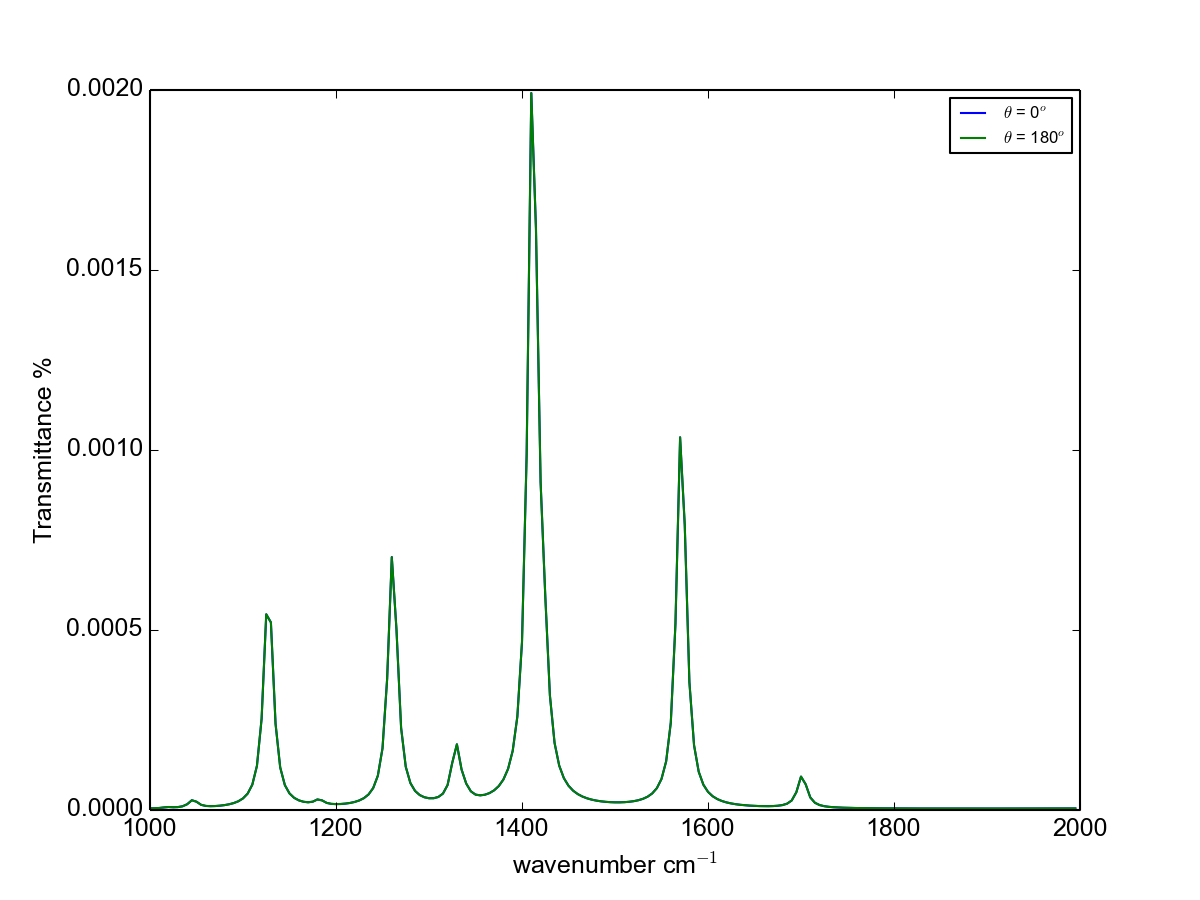
\includegraphics[scale=0.7]{Figures/Ala_candidates_plotting_raman_zz_2.png}
\caption{Raman zz projection spectrum for Alanine Candidate with $\theta$ of $0^{\circ}$ is identical to Alanine Candidate with $\theta$ of $180^{\circ}$} \label{fig:5.8}
\end{figure}

\begin{figure}[!ht] 
\centering
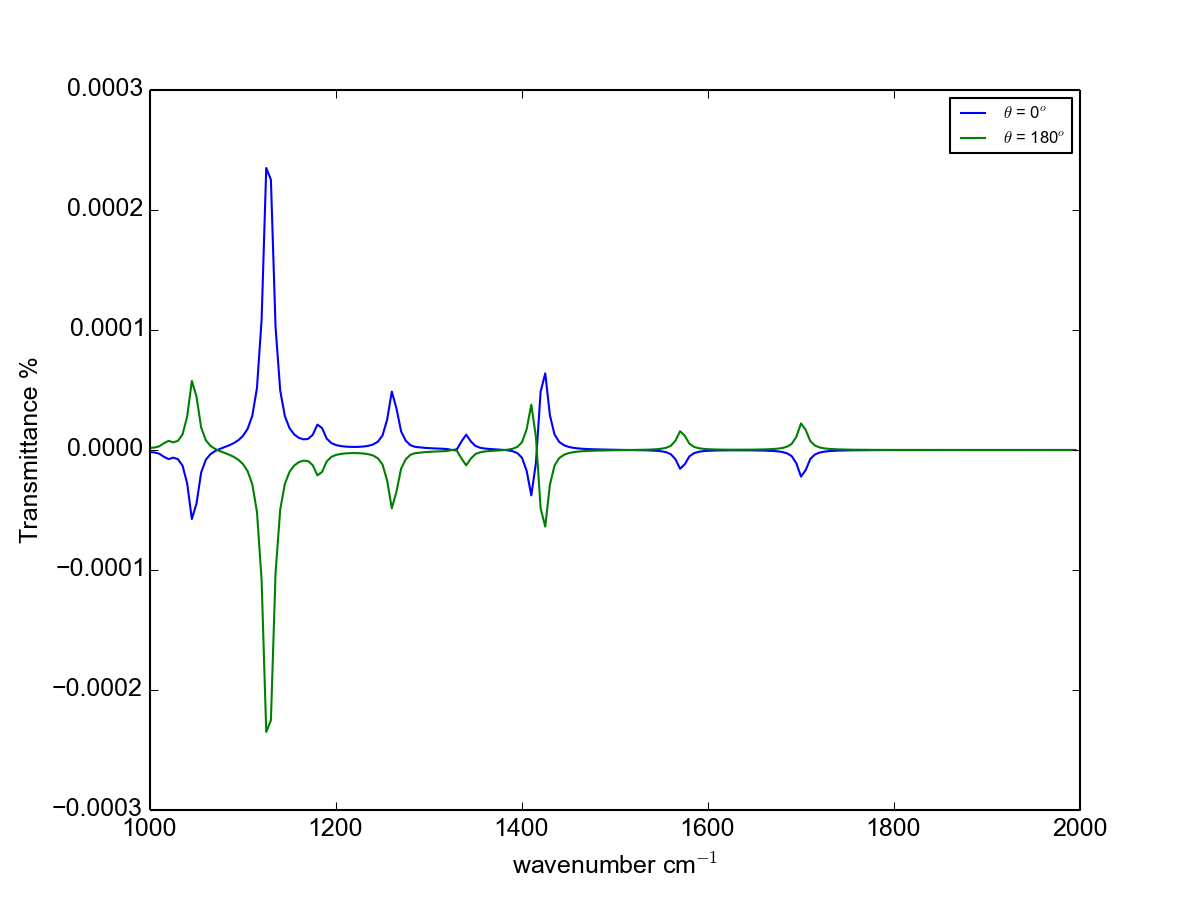
\includegraphics[scale=0.7]{Figures/Ala_candidates_plotting_sfg_zzz_2.png}
\caption{SFG zzz projection spectrum for Alanine Candidate with $\theta$ of $0^{\circ}$ is not identical to Alanine Candidate with $\theta$ of $180^{\circ}$, but symmetric along wavelength} \label{fig:5.9}
\end{figure}
